\subsection*{Redigering af brugeroplysninger} \label{sec:redigrering}
Brugeren kan ud fra app'ens hovedmenu have mulighed for at redigere adgangskode samt sygdomsspecifikke oplysninger. Dette er med henblik på, at brugeren selv skal kunne ændre sin adgangskode samt sin kategorisering, hvis deres helbred forbundet med KOL ændres. Af \autoref{fig:Redigerbrugeroplysninger} er aktivitetsdiagrammet for redigering af brugeroplysninger illustreret. 

\begin{figure}[H]
\centering
\textbf{Aktivitetsdiagram: Redigering af brugeroplysninger}\par\medskip
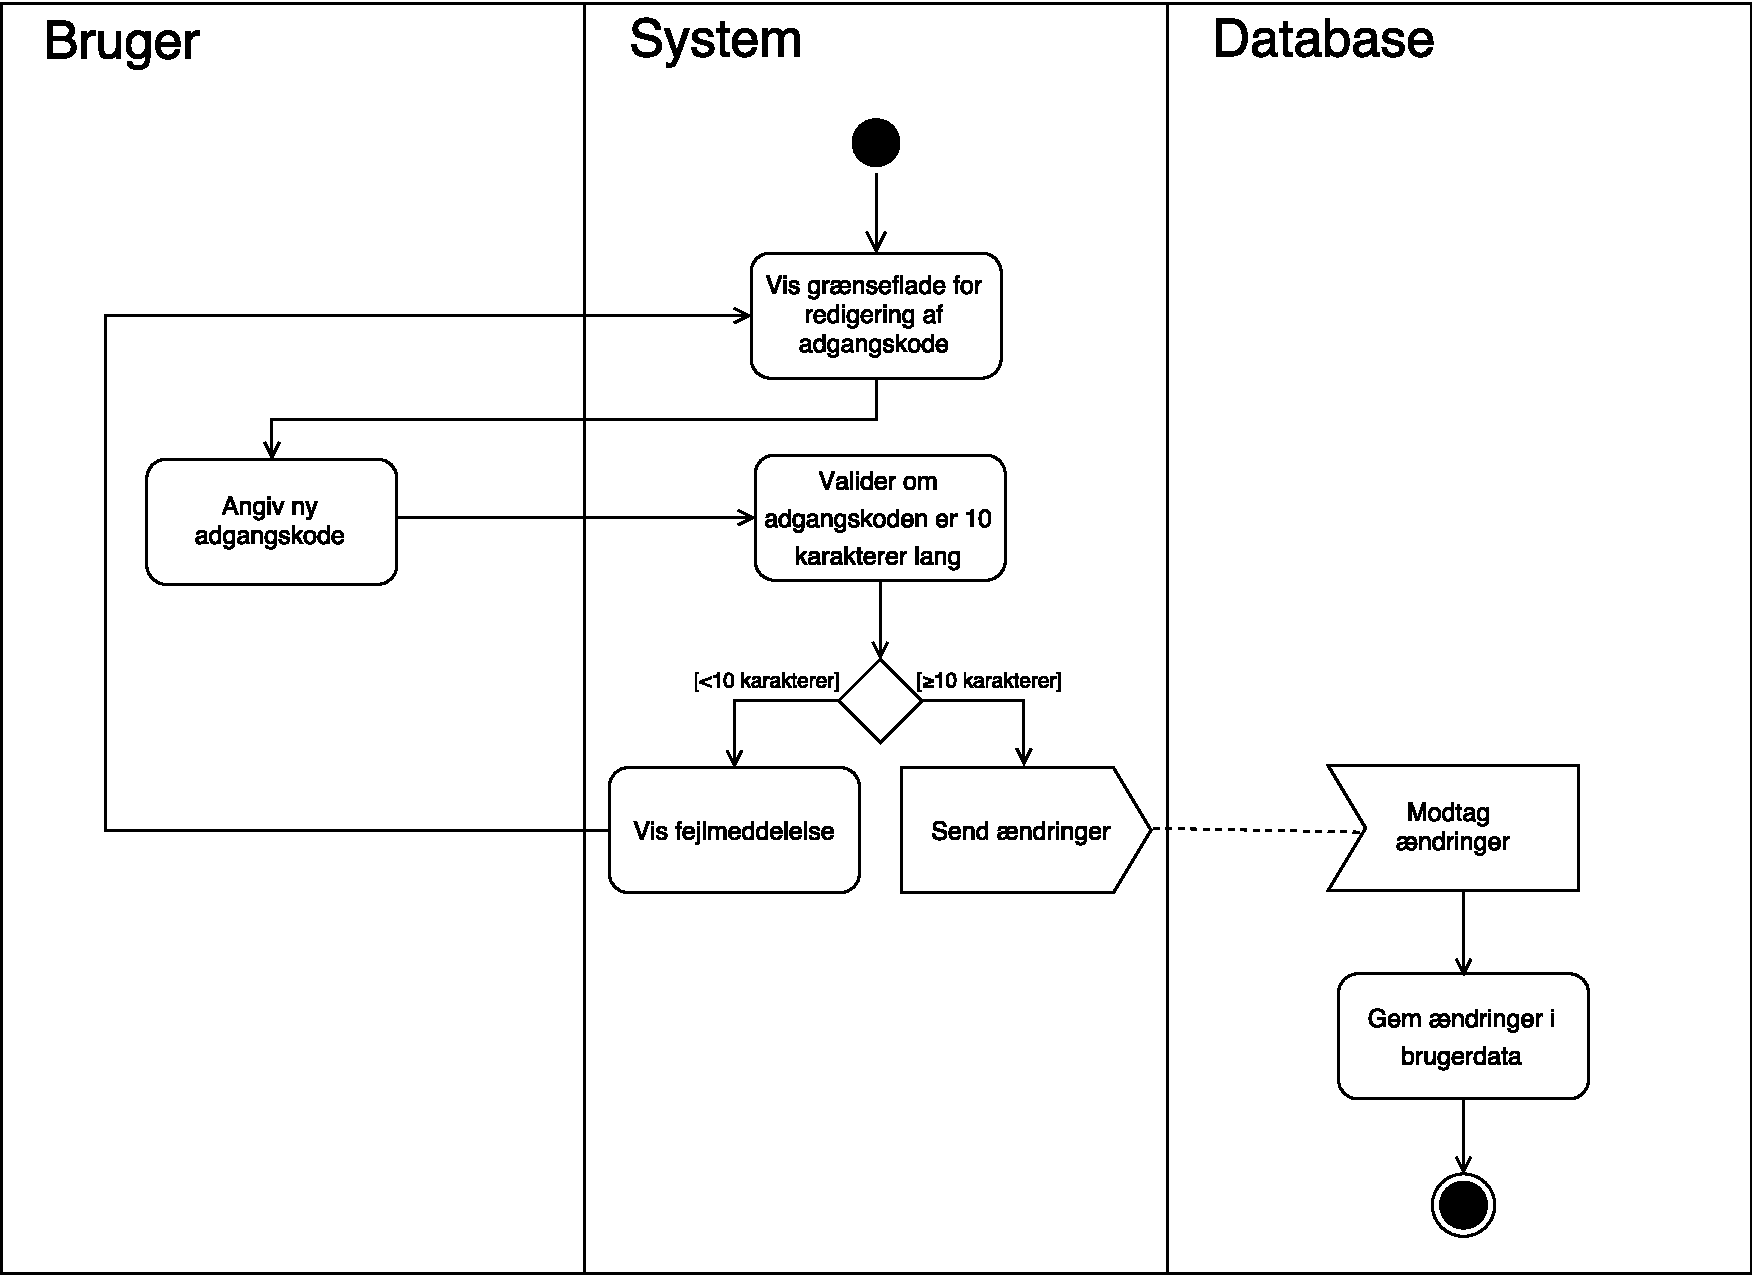
\includegraphics[width=0.9\textwidth]{figures/aktivitetsdiagram/Redigerbrugeroplysninger}
\caption{Aktivitetsdiagram for redigering af brugeroplysninger. Kategorisering af KOL uddybes af \autoref{fig:Kate}.}
\label{fig:Redigerbrugeroplysninger}
\end{figure}

\noindent
Det skal både være muligt at ændre sin adgangskode samt kategoriseringen, som blev defineret i forbindelse med registrering af brugeren. Da brugeren får tildelt en tilfældig adgangskode, skal det være muligt at ændre denne til en personlig adgangskode. For at kunne foretage en ændring af adgangskoden, skal den nye adgangskode som minimum være 10 karakterer lang. Grunden til dette er, at der ved log ind sendes en fejlmeddelelse, hvis indtastede informationer ikke findes i databasen. Adgangskoden skal derfor ikke kunne forveksles med fejlmeddelelsen. Desuden anbefalder Rådet for Digital Sikkerhed, at adgangskoder bør være minimum 10 karakterer lang, men der er ingen krav om en minimumslængde \citep{sikkerhed2015}.
Hvis kravet om minimum 10 karakterer ikke opfyldes, sendes en fejlmeddelse tilbage til brugeren, hvortil en ny adgangskode skal indtastes. 
I tilfælde af, at brugerens tilstand ændres er det ligeledes muligt at redigere denne. Aktivitetsdiagrammet for kategorisering af KOL fremgår af \autoref{fig:Kate}.
Ved korrekt redigering af brugeroplysningerne sendes ændringerne til databasen, hvorefter de gemmes i databasen.